\documentclass[11pt]{article}

% --- Page and typography -------------------------------------------------
\usepackage{geometry}
\geometry{margin=1in}
\usepackage{amsmath,amssymb}
\usepackage{xcolor}
\usepackage{booktabs}
\usepackage{array}
\usepackage{enumitem}
\usepackage{listings}
\usepackage{tikz}
\usetikzlibrary{positioning,fit,backgrounds,shapes.geometric}
\usepackage[colorlinks=true,linkcolor=blue,urlcolor=teal,citecolor=blue]{hyperref}

% --- Code listings (C#) --------------------------------------------------
\definecolor{codekw}{rgb}{0.10,0.27,0.55}
\definecolor{codestr}{rgb}{0.58,0.10,0.10}
\definecolor{codecom}{rgb}{0.972,0.49,0.49} % unused fallback
\definecolor{codecomment}{rgb}{0.10,0.45,0.20}
\definecolor{codebg}{rgb}{0.972,0.972,0.965}
\definecolor{coderule}{rgb}{0.85,0.85,0.82}

\lstset{
  language={[Sharp]C},
  basicstyle=\ttfamily\small,
  keywordstyle=\color{codekw}\bfseries,
  stringstyle=\color{codestr},
  commentstyle=\color{codecomment}\itshape,
  backgroundcolor=\color{codebg},
  frame=single,
  rulecolor=\color{coderule},
  breaklines=true,
  showstringspaces=false,
  columns=fullflexible,
  keepspaces=true,
  captionpos=b,
  morekeywords={var,record,init,with,readonly,struct,where,static,abstract,
    interface,out,ref,params,nameof,sealed,Span,ReadOnlySpan,ReadOnlyMemory,
    Volatile,Interlocked,Func}
}

\newcommand{\cs}[1]{\lstinline|#1|}
\newcommand{\bigO}{\ensuremath{\mathcal{O}}}

% --- Title ---------------------------------------------------------------
\title{\textbf{A Persistent Finger-Tree Library for .NET}\\[2mm]
  \large Design Notes: Architecture, Algorithms, Concurrency, and Testing}
\author{Tools.DataStructures.FingerTree\\ \texttt{src/DataStructures/FingerTree}}
\date{Created (UTC): 2026-06-13\\[1mm]
  Repository HEAD: \texttt{c05c26c97c0074a3fb581157b57bfad439e79729}}

\begin{document}
\maketitle

\begin{abstract}
This document is a single, navigable tour of \texttt{Tools.DataStructures.FingerTree}: a fully
persistent (immutable, structurally sharing) data-structure library for .NET~10 built on finger trees.
It explains the two engine cores --- a purpose-tuned catenable deque and a general monoid-measured
tree --- the lazy-memoized spine that makes their amortized bounds survive branching persistence in a
strict language, the static-abstract ``typeclass'' encoding of measures and predicates, the
allocation-free and closure-free read/split path, the collection and rope families built on top, and
the memory-model argument for safe lock-free concurrent reads. It closes with the three-tier testing
strategy --- example tests, generative property tests, and generative \emph{command-sequence} tests
with shrinking --- plus the tearable-struct concurrency stress suite and the review evidence that backs
the correctness claims. It is written to be read top to bottom by a newcomer and dipped into by a
maintainer.
\end{abstract}

\tableofcontents
\bigskip
\hrule
\bigskip

% =========================================================================
\section{Orientation}
\label{sec:orientation}

The library lives in one project, \texttt{Tools.DataStructures.FingerTree} (namespace identical),
targeting .NET~10 with C\# preview features (static abstract interface members in particular). Every
public type is \textbf{immutable and persistent}: an operation never mutates its receiver; it returns a
new version that shares all unchanged structure with the old one. Old versions remain valid forever,
which is what makes snapshots, undo histories, and lock-free sharing fall out for free
(Section~\ref{sec:concurrency}).

The design rests on a deliberate split into \textbf{two engine cores}, mirroring the Haskell ecosystem's
own split between \texttt{Data.Sequence} (a tuned size-only sequence) and \texttt{Data.FingerTree} (a
general measured tree):

\begin{itemize}[leftmargin=1.4em]
  \item \textbf{The tuned deque} --- \cs{FingerTreeDeque<T>} --- a simplified Claessen-style 2--3 finger
    tree specialized to the size measure, with hand-optimized digit handling. It is the workhorse
    sequence: push/pop both ends, index, split, concat, and a sorted-search surface.
  \item \textbf{The general measured tree} --- \cs{FingerTree<TElement, TMeasure, TMeasureOps>} --- the
    full Hinze--Paterson construction parameterized by an arbitrary monoidal measure. One
    monotone-predicate \cs{Split} specializes it into a priority queue, an ordered search tree, an
    order-statistic tree, an interval index, or a weighted-selection structure, depending only on the
    measure plugged in.
\end{itemize}

On top of those cores sit a measure framework (Section~\ref{sec:measures}), a closure-free predicate API
(Section~\ref{sec:predicates}), a collection family (Section~\ref{sec:collections}), and a rope family
(Section~\ref{sec:ropes}). Table~\ref{tab:complexity} summarizes the headline complexities; the rest of
the document explains how they are achieved and preserved.

% =========================================================================
\section{Background: finger trees in one page}
\label{sec:background}

A finger tree is a functional sequence representation that gives amortized constant-time access to both
ends and logarithmic split/concat/index. The shape is recursive: a tree is either empty, a single
element, or a \emph{deep} node holding a \emph{prefix} digit (1--4 elements), a \emph{middle} subtree
one level deeper whose elements are 2--3-element \emph{nodes}, and a \emph{suffix} digit (1--4 elements).

\begin{figure}[h]
\centering
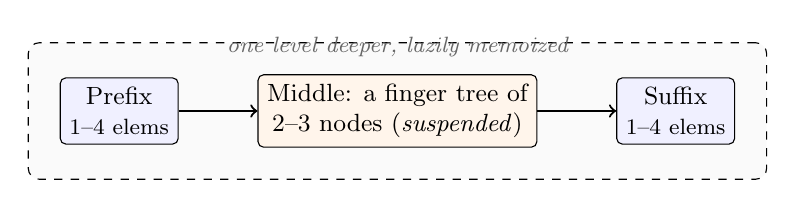
\begin{tikzpicture}[
  box/.style={draw, rounded corners=2pt, minimum height=8mm, align=center, font=\small},
  lab/.style={font=\footnotesize\itshape, text=black!60}]
  \node[box, fill=blue!6] (pre) {Prefix\\ \footnotesize 1--4 elems};
  \node[box, fill=orange!8, right=10mm of pre, minimum width=34mm] (mid)
    {Middle: a finger tree of\\ 2--3 nodes (\emph{suspended})};
  \node[box, fill=blue!6, right=10mm of mid] (suf) {Suffix\\ \footnotesize 1--4 elems};
  \node[lab, above=1mm of mid] {one level deeper, lazily memoized};
  \draw[->, thick] (pre.east) -- (mid.west);
  \draw[->, thick] (mid.east) -- (suf.west);
  \begin{scope}[on background layer]
    \node[draw, dashed, rounded corners, fit=(pre)(mid)(suf), inner sep=4mm, fill=black!2] {};
  \end{scope}
\end{tikzpicture}
\caption{A \emph{deep} finger-tree node. Endpoint access touches only the digits ($\bigO(1)$); the
middle subtree is reached only when an operation descends, and in this library it is a memoized
suspension (Section~\ref{sec:lazy}).}
\label{fig:deep}
\end{figure}

The amortization argument is the classic one: a push/pop that overflows or underflows a digit pays to
repair the spine, but the repaired digits ``bank'' enough slack that the cost is constant on average.
Crucially, that argument assumes the repair is performed \emph{lazily and memoized} --- otherwise a
program that re-runs an operation on a retained old version pays the worst case every time, and the
amortized bound collapses under persistence. Section~\ref{sec:lazy} is about getting that right in a
strict language.

For the underlying theory the repository bundles the two canonical sources next to this document: Hinze
and Paterson's original paper and Claessen's simplified re-explanation (both as PDFs under
\texttt{docs/}). This section is only enough to make the design notes self-contained.

% =========================================================================
\section{Core I: the tuned deque}
\label{sec:deque}

\cs{FingerTreeDeque<T>} is the size-measured sequence. Internally it follows Claessen's simplification:
nodes carry a cached subtree \cs{Size}, digits are small arrays, and the deep constructor is ``smart''
(it rebalances overflowing/underflowing digits using the paper's \emph{chop} on pulls). The public
surface is large and ergonomic:

\begin{itemize}[leftmargin=1.4em, itemsep=1pt]
  \item Endpoints: \cs{AddFirst}, \cs{AddLast}, \cs{RemoveFirst}, \cs{RemoveLast}, \cs{First}, \cs{Last},
    and \cs{TryPeek}/\cs{TryPop} variants.
  \item Positional: \cs{this[int]}, \cs{SetItem}, \cs{InsertAt}, \cs{RemoveAt}, \cs{InsertRange},
    \cs{RemoveRange}, \cs{GetRange}, \cs{SplitAt}, \cs{SplitItemAt}, \cs{SplitRange}.
  \item Catenation: \cs{Concat}, \cs{AddRange}.
  \item Sorted surface (caller maintains order): \cs{SortedLowerBound}, \cs{SortedUpperBound},
    \cs{SortedBinarySearch} (deterministic first-equal duplicate semantics), \cs{SortedContains},
    \cs{SplitAtSortedLowerBound}/\cs{UpperBound}/\cs{EqualRange}, \cs{InsertSorted},
    \cs{RemoveAllSorted}. These exploit cached rightmost-element ``signposts'' to skip whole subtrees.
\end{itemize}

It implements \cs{IReadOnlyList<T>} and exposes a struct enumerator. The complexity profile is the
finger-tree standard: $\bigO(1)$ worst-case endpoint reads, $\bigO(1)$ amortized / $\bigO(\log n)$
worst-case endpoint updates, $\bigO(\log(\min(n,m)))$ concat, and $\bigO(\log(\min(k, n-k)))$
split/index (Table~\ref{tab:complexity}).

% =========================================================================
\section{Core II: the general measured tree}
\label{sec:measured}

\cs{FingerTree<TElement, TMeasure, TMeasureOps>} is the Hinze--Paterson construction. Instead of a
hard-wired size, every node caches a \emph{measure} drawn from a user-supplied commutative-or-not
monoid, and the headline operation is a monotone-predicate split:

\begin{lstlisting}
// Split at the first point where the accumulated measure satisfies the predicate.
(FingerTree<E,M,Ops> Left, FingerTree<E,M,Ops> Right) Split(Func<M,bool> predicate);

// Split around the boundary element, returning it separately.
bool TrySplitFind(Func<M,bool> predicate, out left, out E found, out right);

// Read-only locate: find the boundary element without building result trees.
bool TryLocate(Func<M,bool> predicate, out M measureBefore, out E found);
\end{lstlisting}

The same code becomes different data structures purely by choice of measure:

\begin{center}
\begin{tabular}{@{}ll@{}}
\toprule
\textbf{Measure} & \textbf{Structure it induces} \\
\midrule
size (count)                 & positional sequence / order-statistic indexing \\
$\max$ of a priority         & priority queue (\cs{Split} locates the maximum) \\
last-key (rightmost key)     & ordered search tree (lower/upper-bound split) \\
size $\times$ last-key       & order-statistic ordered tree \\
sum (generic-math)           & cumulative-weight / weighted-selection structure \\
$\max$ interval high-endpoint& interval / stabbing index \\
\bottomrule
\end{tabular}
\end{center}

The two cores are kept separate on purpose. The deque can subtract sizes (the size monoid is a group),
which enables worst-case-cheaper tricks; a general monoid has no inverse, so the measured tree must take
a different route to persistence-robust amortization (Section~\ref{sec:lazy}). Fusing them would
pessimize the common size-only case, exactly the reason the Haskell ecosystem ships both
\texttt{Data.Sequence} and \texttt{Data.FingerTree}.

% =========================================================================
\section{The lazy-memoized spine}
\label{sec:lazy}

This is the load-bearing idea of the whole library, so it gets its own section.

\subsection{The strict-language problem}

The finger-tree amortized bounds depend on the middle subtree being computed lazily and the result being
shared. In Haskell that is automatic: thunks are memoized by the runtime. In a strict language like C\#,
a naive port forces the middle eagerly, so re-running an operation on a \emph{retained} version repeats
the full repair --- and a program that branches off one old version $k$ times pays $k$ times the worst
case. The amortized analysis silently becomes a worst-case-per-branch analysis. Persistence breaks it.

\subsection{Suspensions, memoized with compare-exchange}

The fix follows Hinze and Paterson's strict-language recipe (\S3.2 of the paper, as re-explained by
Claessen): suspend only the middle subtree of each deep node, and memoize the forced result. The library
realizes this with a small explicit cell. For the deque it is \cs{MiddleTree}/\cs{LazyMiddle}/
\cs{PendingMiddle}; for the measured tree it is the parallel
\cs{MeasuredMiddle}/\cs{LazyMeasuredMiddle}/\cs{PendingMeasured}. The cell holds either the pending
operation or, once forced, the computed tree, and publishes the transition atomically:

\begin{lstlisting}
public MeasuredTree<...> Force()
{
    var state = Volatile.Read(ref _state);
    if (state is MeasuredTree<...> computed) return computed;        // already forced
    var result = ((PendingMeasured<...>)state).Run();               // compute (pure)
    var witnessed = Interlocked.CompareExchange(ref _state, result, state);
    return ReferenceEquals(witnessed, state) ? result : (MeasuredTree<...>)witnessed;
}
\end{lstlisting}

Pending operations are \emph{pure}: running one twice yields structurally identical trees. That is what
makes the compare-exchange race benign --- two threads may both force, but they compute the same answer
and exactly one wins publication; the loser adopts the winner's result. No reader can observe a
partially built node. This is also the foundation of the thread-safety claim in
Section~\ref{sec:concurrency}.

\subsection{Depth-1 suspensions: forcing the source}

A subtlety the paper flags: if a push suspension captured \emph{another} suspension as its source, forcing
would cascade a chain of arbitrary length. The library follows the paper's discipline --- the creator of
a push/pop pending operation \emph{forces its source first}, so each suspension is exactly one deferred
operation deep. Forcing therefore recurses only down the tree's $\bigO(\log n)$ depth, never along an
unbounded chain, and the amortized analysis is unaffected.

\subsection{Why the measured tree also memoizes its measure}

For the deque, the measure is size, and a popped subtree's size is recovered by subtraction --- so the
owning node's size is known without forcing. A general monoid has \emph{no inverse}: the measure of a
pop suspension cannot be recovered by subtracting the removed node. Consequently each
\cs{DeepMeasuredTree} memoizes its own measure lazily, in a boxed cell published by compare-exchange:

\begin{lstlisting}
public override TMeasure Measure
{
    get
    {
        if (Volatile.Read(ref _measureBox) is { } existing) return (TMeasure)existing;
        var measure = TMonoid.Combine(TMonoid.Combine(CombineAll(Prefix), _middle.Measure),
                                      CombineAll(Suffix));
        var witnessed = Interlocked.CompareExchange(ref _measureBox, (object)measure!, null);
        return witnessed is null ? measure : (TMeasure)witnessed;
    }
}
\end{lstlisting}

A push suspension can still answer its measure arithmetically (the monoidal sum of its forced source and
the pushed node) without forcing the structure; only a pop suspension must force. The net consequence,
adjudicated in the repository's API-specification defect report, is the \emph{one} place the measured
tree differs from the deque: \cs{Measure} is $\bigO(1)$ \emph{amortized} (not worst-case), while
\cs{First}/\cs{Last} stay $\bigO(1)$ worst-case because they never force the spine. A regression test
pins that endpoint reads never force a suspended spine.

% =========================================================================
\section{The measure framework}
\label{sec:measures}

Measures are encoded with C\#'s static abstract interface members --- a lightweight ``typeclass''
mechanism that keeps the monoid operations as static, devirtualizable calls on a value-type witness, with
no per-element delegate or allocation.

\begin{lstlisting}
public interface IMonoid<TMeasure>
{
    static abstract TMeasure Empty { get; }
    static abstract TMeasure Combine(TMeasure left, TMeasure right);
}

public interface IMeasure<TElement, TMeasure> : ... // Empty, Measure(element), Combine
{
    static abstract TMeasure Measure(TElement element);
}
\end{lstlisting}

Because \cs{TMeasureOps} is a type parameter constrained to the interface, the JIT monomorphizes each
instantiation and the measure calls inline --- the abstraction is free at run time.

\paragraph{Ready-made measures.} \cs{SizeMeasure<T>}, \cs{MaxMeasure}/\cs{MinMeasure}, \cs{KeyMeasure},
and \cs{OrderStatisticMeasure} (with \cs{Optional}/\cs{RankedKey} carriers) cover the common cases. A
custom-order strategy \cs{IComparison<T>} (with \cs{DefaultComparison}/\cs{ReverseComparison}) lets the
ordered structures take a compile-time comparison witness as well.

\paragraph{Sum measure.} \cs{SumMeasure<T>} is a generic-math (\cs{INumber<T>}) persistent
Fenwick-like structure: \cs{SplitByCumulativeWeight} and \cs{TrySelectByCumulativeWeight} give weighted
selection and sampling in $\bigO(\log n)$ over \cs{int}, \cs{double}, \cs{BigInteger}, and any numeric
type.

\paragraph{Product combinator.} \cs{ProductMeasure<...>} pairs two measures into a \cs{MeasurePair}
carrier whose monoid combines component-wise. Named operations (\cs{SplitByFirst}/\cs{SplitBySecond} and
the size$+$sum / size$+$max / size$+$min pairings via the \cs{ProductMeasures} factory) infer all the
type arguments, so callers write a clean call and get, for example, an order-statistic \emph{and}
cumulative-weight structure at once. Product measures nest, so three-component measures compose without
new code.

% =========================================================================
\section{Closure-free reads and splits}
\label{sec:predicates}

A measure query is a monotone predicate over the accumulated measure. Expressed as a \cs{Func<M,bool>}
it allocates a closure on every call --- death by a thousand cuts on a hot read path. The library
therefore makes the predicate a \emph{value-type strategy}, mirroring the measure typeclass:

\begin{lstlisting}
public interface IMeasurePredicate<TMeasure>
{
    bool Invoke(TMeasure measure);
}

// Generic over the predicate's *type*, so the JIT monomorphizes and inlines it: no closure, no boxing.
public bool TryLocate<TPredicate>(TPredicate predicate, out TMeasure before, out TElement found)
    where TPredicate : struct, IMeasurePredicate<TMeasure>;
\end{lstlisting}

The descent itself avoids rebuilding result trees on reads: \cs{LocateTree}/\cs{LocateBuffer} mirror the
\cs{SplitTree}/\cs{SplitBuffer} machinery but only walk to the boundary element. Both the read path
(\cs{TryLocate}) and the split/mutate path (\cs{Split}, \cs{TrySplitFind}) are generic over the struct
predicate; the \cs{Func} overloads simply wrap the delegate in a \cs{FuncMeasurePredicate} adapter for
convenience. The collections route their hot operations through the internal struct predicates
(\cs{CountAbovePredicate}, \cs{KeyAtLeast}, \cs{PriorityFrontPredicate}, \cs{MaxHighAtLeast}, $\dots$),
so they are closure-free throughout.

The payoff is measured, not asserted. \cs{SortedSet.Contains} on $10^5$ elements:

\begin{center}
\begin{tabular}{@{}lrr@{}}
\toprule
\textbf{Implementation path} & \textbf{Time} & \textbf{Allocation} \\
\midrule
\cs{Split}-based (builds result trees) & 2{,}612 ns & 2{,}400 B \\
\cs{TryLocate} with a \cs{Func} lambda & 351 ns & 96 B \\
\cs{TryLocate} with a struct predicate & $\sim$410 ns & \textbf{0 B} \\
\bottomrule
\end{tabular}
\end{center}

The predicate interface is public, so callers can write their own zero-allocation queries against a raw
tree; the library's own predicates stay internal.

% =========================================================================
\section{The collection family}
\label{sec:collections}

These are thin, ergonomic types built on the general core by choosing a measure and routing reads through
struct predicates. All inherit full persistence.

\begin{itemize}[leftmargin=1.4em, itemsep=1pt]
  \item \cs{SortedBag<T>}, \cs{SortedSet<T>}, \cs{SortedDictionary<TKey,TValue>} --- ordered, navigable
    (floor/ceiling/lower/higher), order-statistic indexable, range-extracting, with full set algebra on
    the set. Runtime \cs{IComparer} support; the empty instance collapses to a shared singleton only
    when both empty and default-compared.
  \item \cs{PriorityQueue<TElement,TPriority>} --- meldable, minimum-first, FIFO-stable.
  \item \cs{IntervalTree<T>} --- overlap and point-stabbing queries, overlap counting, value-equal
    membership/removal with duplicates, and coalescing.
  \item \cs{ReversibleDeque<T>} --- the deque's sibling with \textbf{$\bigO(1)$ \cs{Reverse}} via a
    per-node reversal bit and an $\bigO(1)$ \cs{Mirror}; orientation-aware accessors keep even
    mixed-orientation \cs{Concat} at $\bigO(\log\min)$. It is a separate type so its higher constant
    factor falls only on callers who opt in.
\end{itemize}

% =========================================================================
\section{The rope family}
\label{sec:ropes}

A rope is a persistent sequence chunked for locality: leaves hold contiguous runs rather than single
elements, so bulk text-like workloads get cache-friendly storage and $\bigO(1)$ structural slicing while
keeping logarithmic edits.

\begin{itemize}[leftmargin=1.4em, itemsep=1pt]
  \item \cs{Rope<T>} --- element-agnostic positional rope. A \cs{Chunk<T>} is a \cs{ReadOnlyMemory<T>}
    plus a cached length; leaves of a \cs{FingerTree<Chunk<T>, int, ...>} measured by total element
    count. Index $i$ locates the first chunk whose cumulative length exceeds $i$ (a zero-allocation
    \cs{TryLocate}), then offsets within it. A chunk-size policy (min~256, max~2048) splits on growth and
    coalesces on shrink and at concat boundaries to keep chunks healthy.
  \item \cs{MeasuredRope<T,TMeasure,TMeasureOps>} --- the measure-navigable sibling. Each chunk caches a
    combined user measure; the tree is measured by the product \cs{MeasurePair<int,TMeasure>} (count
    \emph{and} user measure). Positional operations run on the count component; \cs{Measure},
    \cs{PrefixMeasure}, \cs{SplitByMeasure}, and \cs{TryLocateByMeasure} navigate the user measure in
    $\bigO(\log n)$ with a bounded within-chunk scan.
  \item \cs{RopeText} --- a companion extension layer that keeps the cores element-agnostic while making
    text ergonomic: a ready-made \cs{NewlineMeasure}, string interop, $\bigO(\log n)$ line/column
    navigation (offset $\leftrightarrow$ (line, column), \cs{GetLine}, \cs{Lines}), and a forward-only
    \cs{TextReader} adapter.
\end{itemize}

Editing a $10^6$-element rope is $\sim$2--3 orders of magnitude faster than the equivalent \cs{string}
rebuild and flat across size (logarithmic, kilobytes not megabytes); line navigation on a million-line
buffer is thousands of times faster than a linear scan. The curated numbers and their honest
counterpoints live in \texttt{docs/benchmarks.md}.

% =========================================================================
\section{Persistence and concurrency}
\label{sec:concurrency}

\subsection{Snapshots and undo are free}

Keeping a snapshot is keeping a reference --- $\bigO(1)$, zero allocation, never invalidated because
nothing mutates it. An edit allocates only the $\bigO(\log n)$ of structure that actually changes; the
rest is shared. An undo/redo history is therefore a cursor over retained versions, needing no diffing and
no inverse operations. A thousand versions cost a thousand small deltas, not a thousand copies.

\subsection{Lock-free concurrent reads, and a memory-model argument}

Because a version is immutable, any number of threads may read it concurrently with no locks. A
producer/consumer setup needs only an atomic publish of a single reference: the producer builds the next
version privately and stores it with one volatile write; consumers read that reference and operate on the
complete snapshot they captured. No consumer ever sees a half-applied edit.

The subtler claim is that even \emph{first} reads of a freshly built structure are safe, including when
the element type \cs{T} or the measure type \cs{TMeasure} is a multi-word struct that the runtime copies
non-atomically (a candidate for \emph{torn} reads). The argument, audited in a dedicated review round:

\begin{itemize}[leftmargin=1.4em, itemsep=1pt]
  \item Element and child storage lives in \cs{readonly} arrays (the deep node's \cs{Prefix}/\cs{Suffix},
    the chunk arrays). They are written once at construction and never mutated; the .NET memory model's
    \cs{readonly}-field freeze plus safe publication of the immutable object graph makes their contents
    visible before any reader obtains the reference --- even on a weak memory model such as ARM.
  \item Every \emph{mutable} cell holds a \emph{reference} (\cs{object}): the suspension \cs{_state} and
    the boxed \cs{_measureBox}. They are read with \cs{Volatile.Read} and published with
    \cs{Interlocked.CompareExchange}, so a large \cs{TMeasure} is boxed and published \emph{atomically} ---
    a reader unboxes a stable box and can never observe a torn field.
  \item No code path reads an unboxed multi-word \cs{T}/\cs{TMeasure} from a location another thread can
    concurrently write. Therefore no torn or partially initialized read is possible for any element or
    measure type.
\end{itemize}

This is not merely ``safe once warmed up'': it is safe to share \emph{immediately}, including the lazy
work the amortized bounds depend on. The full worked patterns are in
\texttt{docs/persistence-and-concurrency.md}.

% =========================================================================
\clearpage
\section{Complexity summary}
\label{sec:complexitysummary}

\begin{table}[ht]
\centering
\renewcommand{\arraystretch}{1.15}
\begin{tabular}{@{}lll@{}}
\toprule
\textbf{Operation} & \textbf{Deque} & \textbf{Measured tree} \\
\midrule
First / Last (read)        & $\bigO(1)$ worst-case          & $\bigO(1)$ worst-case \\
Push / pop an end          & $\bigO(1)$ amortized$^\dagger$ & $\bigO(1)$ amortized$^\dagger$ \\
Measure of whole structure & $\bigO(1)$ (cached size)       & $\bigO(1)$ amortized$^\dagger$ \\
Index / positional split   & $\bigO(\log(\min(k,n{-}k)))$   & --- (size measure) \\
Predicate split / locate   & ---                            & $\bigO(\log(\min(k,n{-}k)))$ amortized \\
Concat                     & $\bigO(\log(\min(n,m)))$       & $\bigO(\log(\min(n,m)))$ \\
Reverse (\cs{ReversibleDeque}) & $\bigO(1)$                 & --- \\
\bottomrule
\end{tabular}
\caption{Headline complexities. $^\dagger$Amortized bounds hold \emph{under fully persistent (branching)
use} because of the lazy-memoized spine (Section~\ref{sec:lazy}); worst-case for those rows is
$\bigO(\log n)$.}
\label{tab:complexity}
\end{table}

% =========================================================================
\section{Testing strategy}
\label{sec:testing}

Correctness is established in three complementary tiers plus a concurrency suite, all in one xUnit project
(293 tests, warning-free with \cs{CS1591} as an error).

\begin{enumerate}[leftmargin=1.6em, itemsep=2pt]
  \item \textbf{Example and unit tests} --- contract tests, edge cases, internal-invariant validation
    (via \cs{InternalsVisibleTo}) after every step of randomized histories, complexity guards that pin
    comparer-call counts and zero-allocation endpoint reads, branching-persistence tests, and worked
    \emph{documentation} examples (snapshots, undo/redo, lock-free reads) that double as runnable proofs
    for the prose in this document.
  \item \textbf{Property-based tests (CsCheck)} --- thousands of generated inputs with shrinking: rope
    edit histories versus a \cs{List} oracle with chunk-invariant checks after every step; split/concat
    and slice laws; text-rope line navigation versus a \cs{string.Split} model with offset round-trips at
    every offset; the sorted collections versus the framework \cs{SortedSet}/\cs{HashSet} and a multiset
    model.
  \item \textbf{Model-based command-sequence tests (CsCheck \cs{SampleModelBased})} --- generate
    sequences of \emph{operations} (not just data) for the deque, rope, measured tree, measured rope, and
    sorted set, replay each against a reference model checking equivalence after every step, and shrink a
    failure to a \emph{minimal failing program} rather than a minimal input. Each immutable structure is
    wrapped in a mutable cell so an operation can rebind the current version. The per-step check also
    verifies the full read/split surface at every reached state: the sorted deque's binary search and its
    three sorted splits, the measured tree's locate/split-find, and the sorted set's navigable queries.
\end{enumerate}

\paragraph{Concurrency stress.} A dedicated suite uses a deliberately \emph{tearable} 32-byte struct
(four longs that must always agree; an \cs{IsIntact} predicate detects any torn read) as \emph{both}
element and measure, under shared concurrent reads, concurrent first reads that force the lazy measure
boxes, lock-free sliding-window publication, and a long-running branch-and-read soak (duration tunable via
the \cs{FINGERTREE_STRESS_SECONDS} environment variable). These empirically corroborate the memory-model
argument of Section~\ref{sec:concurrency}: zero tears across a multi-second soak.

\paragraph{Adversarial review and mutation evidence.} The concurrency code and the tests were each put
through read-only review rounds (a memory-model lens that found the design sound under weak memory, a
harness-correctness lens, and a test-soundness lens whose one confirmed finding --- a range-removal
generator biased to a no-op --- was fixed). The model-based harness was further validated by
\emph{mutation testing}: deliberately breaking a model operation made the suite fail and shrink to a
two-operation counterexample (\cs{[RemoveLast, AddFirst 50]}), and corrupting a split expectation shrank
to \cs{[InsertSorted 10]} --- direct evidence the tests are not vacuous and that shrinking yields
readable minimal programs.

% =========================================================================
\section{Repository map}
\label{sec:map}

\begin{itemize}[leftmargin=1.4em, itemsep=1pt]
  \item \texttt{src/Tools.DataStructures.FingerTree/} --- the library. \cs{FingerTreeDeque} and its
    \texttt{Internal/} core (\cs{Tree}, \cs{Digit}, \cs{Node}, \cs{MiddleTree}, \cs{TreeOperations});
    \cs{FingerTree} and \texttt{Internal/Measured/}; the measure framework (\cs{Measures},
    \cs{BuiltInMeasures}, \cs{SumMeasure}, \cs{ProductMeasure}, \cs{Comparisons}); the predicate API
    (\cs{MeasurePredicate}, \cs{Internal/MeasurePredicates}); the collections; and the rope family
    (\cs{Rope}, \cs{MeasuredRope}, \cs{RopeText}).
  \item \texttt{tests/Tools.DataStructures.FingerTree.Tests/} --- the three-tier xUnit suite plus the
    tearable concurrency stress tests.
  \item \texttt{benchmarks/} --- the BenchmarkDotNet harness; curated results in
    \texttt{docs/benchmarks.md}.
  \item \texttt{docs/} --- this document, the normative API specification and its defect report, the
    persistence/concurrency guide, the benchmark write-up, and the bundled source papers.
\end{itemize}

% =========================================================================
\section{References}
\label{sec:references}

\begin{enumerate}[leftmargin=1.6em, itemsep=1pt]
  \item R. Hinze and R. Paterson. \emph{Finger trees: a simple general-purpose data structure}. Journal
    of Functional Programming, 2006. (Bundled: \texttt{docs/Finger trees - a simple general-purpose data
    structure.pdf}.)
  \item K. Claessen. \emph{Finger Trees Explained Anew, and Slightly Simplified (Functional Pearl)}.
    Haskell Symposium, 2020. (Bundled: \texttt{docs/Finger Trees Explained Anew, and Slightly
    Simplified.pdf}.)
  \item Repository documents: \texttt{docs/api-specification.md},
    \texttt{docs/api-specification-defect-report-complexity-guarantees.md},
    \texttt{docs/persistence-and-concurrency.md}, \texttt{docs/benchmarks.md}.
\end{enumerate}

\end{document}
